\chapter{Bootstrap Sampling}\label{bootstrap-sampling}

In the previous chapter we used resampling to compute standard errors
and confidence intervals, which quantify the variability in an estimate
due to random sampling.

In this chapter, we'll use data from the General Social Survey (GSS) to
estimate average income and the 10th percentile of income. We'll see
that the resampling method we used in the previous chapter works for the
average income but not for the 10th percentile.

To solve this problem, we'll use another kind of resampling, called
bootstrapping or bootstrap sampling. Then we'll use bootstrapping to
compute sampling distributions and confidence intervals for other
statistics, including the coefficient of correlation and the parameters
of linear regression. Finally, I'll point out a problem with bootstrap
resampling when there are not enough different values in a dataset, and
a way to solve it with KDE resampling.

\section{Estimating Average Income}\label{estimating-average-income}

As a first example, we'll use data from the General Social Survey to
estimate average family income. We'll work with an extract that contains
just the columns we need, as we did in Chapter 8. Instructions for
downloading the extract are in the notebook for this chapter.

We can load the data like this and display the first few rows.

\begin{lstlisting}[language=Python,style=source]
import pandas as pd

gss = pd.read_hdf('gss_extract_2022.hdf', 'gss')
gss.head()
\end{lstlisting}

\begin{tabular}{lrrrrrrrrr}
\midrule
 & year & id & age & educ & degree & sex & gunlaw & grass & realinc \\
\midrule
0 & 1972 & 1 & 23.000000 & 16.000000 & 3.000000 & 2.000000 & 1.000000 & NaN & 18951.000000 \\
1 & 1972 & 2 & 70.000000 & 10.000000 & 0.000000 & 1.000000 & 1.000000 & NaN & 24366.000000 \\
2 & 1972 & 3 & 48.000000 & 12.000000 & 1.000000 & 2.000000 & 1.000000 & NaN & 24366.000000 \\
3 & 1972 & 4 & 27.000000 & 17.000000 & 3.000000 & 2.000000 & 1.000000 & NaN & 30458.000000 \\
4 & 1972 & 5 & 61.000000 & 12.000000 & 1.000000 & 2.000000 & 1.000000 & NaN & 50763.000000 \\
\midrule
\end{tabular}

The column \passthrough{\lstinline!realinc!} records family income,
converted to 1986 dollars. The following figure uses the Seaborn
function \passthrough{\lstinline!kdeplot!} to show the distribution of
family income. The argument \passthrough{\lstinline!cut=0!} cuts off the
curve so it doesn't extend beyond the observed minimum and maximum
values.

\begin{lstlisting}[language=Python,style=source]
import seaborn as sns
import matplotlib.pyplot as plt

sns.kdeplot(gss['realinc'] / 1000, label='GSS data', cut=0)

plt.xlabel('Family income ($1000s)')
plt.ylabel('PDF')
plt.title('Distribution of income')
plt.legend();
\end{lstlisting}

\begin{center}
\includegraphics[width=4in]{chapters/12_bootstrap_files/12_bootstrap_11_0.png}
\end{center}

The distribution of income is skewed to the right; most household
incomes are less than \$60,000, but a few are substantially higher. Here
are the mean and standard deviation of the reported incomes.

\begin{lstlisting}[language=Python,style=source]
mean_realinc = gss['realinc'].mean()
std_realinc = gss['realinc'].std()
print(mean_realinc, std_realinc)
\end{lstlisting}

\begin{lstlisting}[style=output]
32537.399981032493 30883.22609399141
\end{lstlisting}

The average family income in this sample is \$32,537. But if we ran the
GSS survey again, the average might be higher or lower. To see how much
it might vary, we can use this function from the previous chapter to
simulate the sampling process.

\begin{lstlisting}[language=Python,style=source]
import numpy as np

def simulate_sample_mean(n, mu, sigma):
    sample = np.random.normal(mu, sigma, size=n)
    return sample.mean()
\end{lstlisting}

\passthrough{\lstinline!simulate\_sample\_mean!} takes as parameters the
sample size and the mean and standard deviation. It generates a sample
from a normal distribution and returns the mean.

Before we call this function, we have to count the number of valid
responses.

\begin{lstlisting}[language=Python,style=source]
n_realinc = gss['realinc'].notna().sum()
n_realinc
\end{lstlisting}

\begin{lstlisting}[style=output]
64912
\end{lstlisting}

Now, if we call \passthrough{\lstinline!simulate\_sample\_mean!} once,
we get a single value from the sampling distribution of the mean.

\begin{lstlisting}[language=Python,style=source]
simulate_sample_mean(n_realinc, mean_realinc, std_realinc)
\end{lstlisting}

\begin{lstlisting}[style=output]
32573.420195135117
\end{lstlisting}

If we call it many times, we get a random sample from the sampling
distribution.

\begin{lstlisting}[language=Python,style=source]
t1 = [simulate_sample_mean(n_realinc, mean_realinc, std_realinc)
      for i in range(1000)]
\end{lstlisting}

Here's what the sampling distribution looks like.

\begin{lstlisting}[language=Python,style=source]
sns.kdeplot(t1)

plt.xlabel('Family income (1986 $)')
plt.ylabel('PDF')
plt.title('Sampling distribution of mean income');
\end{lstlisting}

\begin{center}
\includegraphics[width=4in]{chapters/12_bootstrap_files/12_bootstrap_24_0.png}
\end{center}

This distribution shows how much we would expect the observed mean to
vary if we ran the GSS survey again. We'll use the following function to
summarize the sampling distribution.

\begin{lstlisting}[language=Python,style=source]
def summarize(t, digits=2, label=''):
    est = np.mean(t).round(digits)
    SE = np.std(t).round(digits)
    CI90 = np.percentile(t, [5, 95]).round(digits)
    data = [est, SE, CI90]
    columns = ['Estimate', 'SE', 'CI90']
    table = pd.DataFrame([data], index=[label], columns=columns)
    return table
\end{lstlisting}

\begin{lstlisting}[language=Python,style=source]
summary1 = summarize(t1, digits=1)
summary1
\end{lstlisting}

\begin{tabular}{lrrl}
\midrule
 & Estimate & SE & CI90 \\
\midrule
 & 32533.900000 & 120.700000 & [32331.3 32724.2] \\
\midrule
\end{tabular}

The result shows the mean of the sampling distribution, the standard
error, and a 90\% confidence interval. The mean of the sampling
distribution is close to the mean of the data, as we expect. The
standard error quantifies with width of the sampling distribution, which
is about \$121. Informally, that's how much we would expect the sample
mean to change if we ran the survey again. And if we ran the survey many
times and computed the average income each time, we would expect 90\% of
the results to fall in the range from 32,331 to 32,724.

In this section, we used a normal distribution to simulate the sampling
process. The normal distribution is not a particularly good model for
the distribution of income, but it works well enough for this example,
and the results are reasonable. In the next section we'll see an example
where the normal distribution is not good enough and the results are not
reasonable. Then we'll see how to fix the problem.

\section{Estimating Percentiles}\label{estimating-percentiles}

Suppose that, instead of estimating the average income, we want to
estimate the 10th percentile. Computing percentiles of income is often
relevant to discussions of income inequality. To compute the 10th
percentile of the data, we can use the NumPy function
\passthrough{\lstinline!percentile!}, but we have to drop the NaN
values.

\begin{lstlisting}[language=Python,style=source]
np.percentile(gss['realinc'].dropna(), 10)
\end{lstlisting}

\begin{lstlisting}[style=output]
5730.0
\end{lstlisting}

The 10th percentile of the sample is \$5730, but if we collected another
sample, the result might be higher or lower. To see how much it would
vary, we can use the following function to simulate the sampling
process: \passthrough{\lstinline!simulate\_sample\_percentile!}
generates a sample from a normal distribution and returns the 10th
percentile.

\begin{lstlisting}[language=Python,style=source]
def simulate_sample_percentile(n, mu, sigma):
    sample = np.random.normal(mu, sigma, size=n)
    return np.percentile(sample, 10)
\end{lstlisting}

If we call it several times, the result is a sample from the sampling
distribution of the 10th percentile.

\begin{lstlisting}[language=Python,style=source]
t2 = [simulate_sample_percentile(n_realinc, mean_realinc, std_realinc)
      for i in range(1000)]
\end{lstlisting}

Here's what that sampling distribution looks like.

\begin{lstlisting}[language=Python,style=source]
sns.kdeplot(t2)

plt.xlabel('Family income (1986 $)')
plt.ylabel('PDF')
plt.title('Sampling distribution of the 10th percentile');
\end{lstlisting}

\begin{center}
\includegraphics[width=4in]{chapters/12_bootstrap_files/12_bootstrap_38_0.png}
\end{center}

We can summarize the results like this.

\begin{lstlisting}[language=Python,style=source]
summary2 = summarize(t2)
summary2
\end{lstlisting}

\begin{tabular}{lrrl}
\midrule
 & Estimate & SE & CI90 \\
\midrule
 & -7035.830000 & 205.950000 & [-7377.78 -6709.29] \\
\midrule
\end{tabular}

We can see that something has gone wrong. All of the values in the
sampling distribution are negative, even though no one in the sample
reported a negative income. To see what happened, let's look at the
distribution of reported incomes again compared to the normal
distribution with the same mean and standard deviation.

\begin{lstlisting}[language=Python,style=source]
from scipy.stats import norm

xs = np.linspace(-50, 150)
ys = norm(mean_realinc/1000, std_realinc/1000).pdf(xs)
\end{lstlisting}

\begin{lstlisting}[language=Python,style=source]
sns.kdeplot(gss['realinc'] / 1000, label='GSS data', cut=0)
plt.plot(xs, ys, color='0.7', label='normal model')

plt.xlabel('Family income ($1000s)')
plt.ylabel('PDF')
plt.title('Distribution of income')
plt.legend();
\end{lstlisting}

\begin{center}
\includegraphics[width=4in]{chapters/12_bootstrap_files/12_bootstrap_43_0.png}
\end{center}

The problem is that the normal model extends past the lower bound of the
observed values, so it doesn't produce sensible results. Fortunately
there is a simple alternative that is more robust: bootstrapping.

\section{Bootstrapping}\label{bootstrapping}

Bootstrapping is a kind of resampling, based on the framework we saw in
the previous chapter:

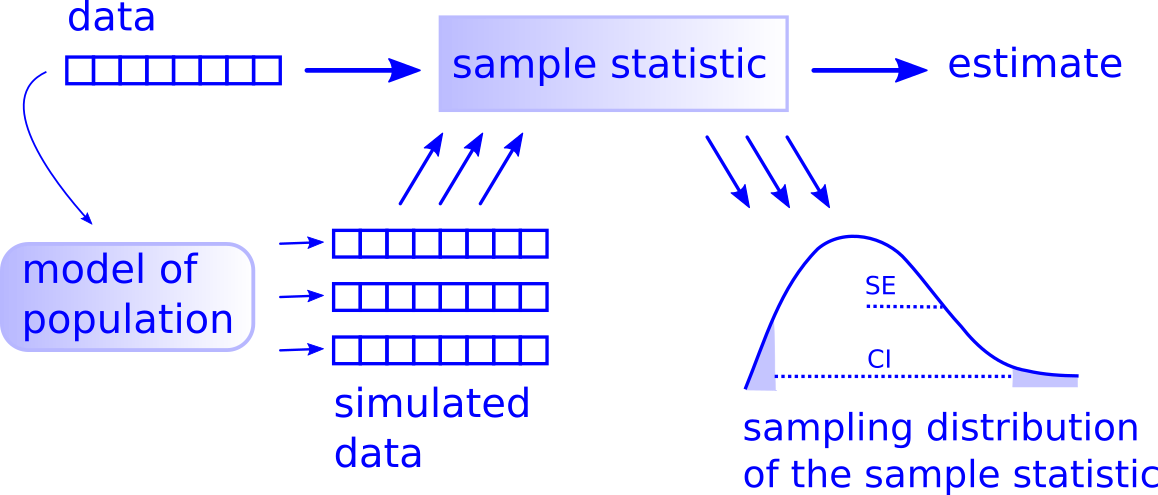
\includegraphics{chapters/figs/resampling.png}

The idea is that we treat the original sample as if it were the entire
population, and simulate the sampling process by choosing random rows
with replacement. \passthrough{\lstinline!DataFrame!} provides a method
called \passthrough{\lstinline!sample!} we can use to select a random
sample of the rows.

\begin{lstlisting}[language=Python,style=source]
bootstrapped = gss.sample(n=n_realinc, replace=True)
bootstrapped.shape
\end{lstlisting}

\begin{lstlisting}[style=output]
(64912, 9)
\end{lstlisting}

The argument \passthrough{\lstinline!n=n\_realinc!} means that the
bootstrapped sample has the same size as the original.
\passthrough{\lstinline!replace=True!} means that sampling is done with
replacement -- that is, the same row can be chosen more than once. To
see how many times each row appears in the bootstrapped sample, we can
use \passthrough{\lstinline!value\_counts!} and the
\passthrough{\lstinline!id!} column, which contains a unique identifier
for each respondent.

\begin{lstlisting}[language=Python,style=source]
repeats = bootstrapped['id'].value_counts()
repeats.head()
\end{lstlisting}

\begin{lstlisting}[style=output]
id
889     51
504     48
1302    47
295     47
524     46
Name: count, dtype: int64
\end{lstlisting}

Several of the rows appear more than 40 times. Since some rows appear
many times, other rows don't appear at all. To see how many, we can use
\passthrough{\lstinline!set!} subtraction to count the values of
\passthrough{\lstinline!id!} that appear in the original dataset but not
the bootstrapped sample.

\begin{lstlisting}[language=Python,style=source]
unused = set(gss['id']) - set(bootstrapped['id'])
len(unused)
\end{lstlisting}

\begin{lstlisting}[style=output]
229
\end{lstlisting}

Now we can use bootstrapping to generate a sampling distribution. For
example, the following function takes a
\passthrough{\lstinline!DataFrame!}, generates a bootstrapped sample,
and returns the average income.

\begin{lstlisting}[language=Python,style=source]
def bootstrap_mean(df, varname):
    bootstrapped = df.sample(n=len(df), replace=True)
    return bootstrapped[varname].mean()
\end{lstlisting}

If we run it many times, we get a sample from the sampling distribution
of the mean.

\begin{lstlisting}[language=Python,style=source]
t3 = [bootstrap_mean(gss, 'realinc')
      for i in range(1001)]
\end{lstlisting}

Here's a summary of the results, compared to the results based on the
normal model.

\begin{lstlisting}[language=Python,style=source]
summary3 = summarize(t3)
table = pd.concat([summary1, summary3])
table.index=['normal model', 'bootstrapping']
table
\end{lstlisting}

\begin{tabular}{lrrl}
\midrule
 & Estimate & SE & CI90 \\
\midrule
normal model & 32533.900000 & 120.700000 & [32331.3 32724.2] \\
bootstrapping & 32541.000000 & 119.320000 & [32342.12 32732.88] \\
\midrule
\end{tabular}

The results from bootstrap sampling are consistent with the results
based on the normal model. Now let's see what happens when we estimate
the 10th percentile.

The following function generates a bootstrapped sample and returns the
10th percentile. Instead of \passthrough{\lstinline!percentile!} from
Numpy, it uses \passthrough{\lstinline!quantile!} from Pandas, which
drops \passthrough{\lstinline!NaN!} values. The parameter of
\passthrough{\lstinline!quantile!} is a probability between 0 and 1,
rather than a percentage between 0 and 100.

\begin{lstlisting}[language=Python,style=source]
def bootstrap_income_percentile(df):
    bootstrapped = df.sample(n=len(df), replace=True)
    return bootstrapped['realinc'].quantile(0.1)
\end{lstlisting}

We can use it to generate a sample from the sampling distribution of the
10th percentile.

\begin{lstlisting}[language=Python,style=source]
t4 = [bootstrap_income_percentile(gss)
      for i in range(1001)]
\end{lstlisting}

Here are the results along with the results based on the normal model.

\begin{lstlisting}[language=Python,style=source]
summary4 = summarize(t4)
table = pd.concat([summary2, summary4])
table.index=['normal model', 'bootstrapping']
table
\end{lstlisting}

\begin{tabular}{lrrl}
\midrule
 & Estimate & SE & CI90 \\
\midrule
normal model & -7035.830000 & 205.950000 & [-7377.78 -6709.29] \\
bootstrapping & 5685.330000 & 91.070000 & [5512.5 5827.5] \\
\midrule
\end{tabular}

The mean of the sampling distribution is consistent with the 10th
percentile of the data, which is \$5631. So the results from
bootstrapping are more sensible than the results based on the normal
model.

In general, bootstrapping is robust -- that is, it works well with many
different distributions and many different statistics. However, at the
end of the chapter, we'll see one example where it fails.

\section{Working with Bigger Data}\label{working-with-bigger-data}

As sample size increases, errors due to random sampling get smaller. To
demonstrate this effect, we'll use data from the Behavioral Risk Factor
Surveillance System (BRFSS) to estimate the average height for men in
the United States.

First, let's read the 2021 data, which I have stored in an HDF file.
Instructions for downloading it are in the notebook for this chapter.

We can read the data like this.

\begin{lstlisting}[language=Python,style=source]
import pandas as pd

brfss = pd.read_hdf('brfss_2021.hdf', 'brfss')
brfss.shape
\end{lstlisting}

\begin{lstlisting}[style=output]
(438693, 10)
\end{lstlisting}

This dataset contains 438,693 rows, one for each respondent, and 10
columns, one for each variable in the extract. Here are the first few
rows.

\begin{lstlisting}[language=Python,style=source]
brfss.head()
\end{lstlisting}

\begin{tabular}{lrrrrrrrrrr}
\midrule
 & SEQNO & HTM4 & WTKG3 & \_SEX & \_AGEG5YR & \_VEGESU1 & \_INCOMG1 & \_LLCPWT & \_HTM4G10 & AGE \\
\midrule
0 & 2021000001 & 150.000000 & 32.660000 & 2 & 11.000000 & 2.140000 & 3.000000 & 744.745531 & 140.000000 & 72.000000 \\
1 & 2021000002 & 168.000000 & NaN & 2 & 10.000000 & 1.280000 & NaN & 299.137394 & 160.000000 & 67.000000 \\
2 & 2021000003 & 165.000000 & 77.110000 & 2 & 11.000000 & 0.710000 & 2.000000 & 587.862986 & 160.000000 & 72.000000 \\
3 & 2021000004 & 163.000000 & 88.450000 & 2 & 9.000000 & 1.650000 & 5.000000 & 1099.621570 & 160.000000 & 62.000000 \\
4 & 2021000005 & 180.000000 & 93.440000 & 1 & 12.000000 & 2.580000 & 2.000000 & 1711.825870 & 170.000000 & 77.000000 \\
\midrule
\end{tabular}

The \passthrough{\lstinline!HTM4!} column contains the respondents'
heights in centimeters.

\begin{lstlisting}[language=Python,style=source]
height = brfss['HTM4']
\end{lstlisting}

To select male respondents, we'll use the \passthrough{\lstinline!SEX!}
column to make a Boolean \passthrough{\lstinline!Series!}.

\begin{lstlisting}[language=Python,style=source]
male = (brfss['_SEX'] == 1)
male.sum()
\end{lstlisting}

\begin{lstlisting}[style=output]
203760
\end{lstlisting}

We can use \passthrough{\lstinline!notna!} and
\passthrough{\lstinline!sum!} to count the number of male respondents
with valid height data.

\begin{lstlisting}[language=Python,style=source]
n_height = height[male].notna().sum()
n_height
\end{lstlisting}

\begin{lstlisting}[style=output]
193701
\end{lstlisting}

Here is the mean and standard deviation of these values.

\begin{lstlisting}[language=Python,style=source]
mean_height = height[male].mean()
std_height = height[male].std()
mean_height, std_height
\end{lstlisting}

\begin{lstlisting}[style=output]
(178.14807357731763, 7.987083970017878)
\end{lstlisting}

The average height for men in the U.S. is about 178 cm. To see how
precise this estimate is, we can use bootstrapping to generate values
from the sampling distribution. To reduce computation time, I set the
number of iterations to 201.

\begin{lstlisting}[language=Python,style=source]
t5 = [bootstrap_mean(brfss[male], 'HTM4')
      for i in range(201)]

summarize(t5, digits=3)
\end{lstlisting}

\begin{tabular}{lrrl}
\midrule
 & Estimate & SE & CI90 \\
\midrule
 & 178.148000 & 0.018000 & [178.12  178.179] \\
\midrule
\end{tabular}

Because the sample size is so large, the standard error is small and the
confidence interval is narrow. This result suggests that our estimate is
very precise, which is true in the sense that the error due to random
sampling is small.

But there are other sources of error. For example, the heights and
weights in this dataset are self-reported, so they are vulnerable to
\textbf{social desirability bias}, which is the tendency of people to
represent themselves in a positive light.

It's also possible that there are errors in recording the data. In a
previous year of the BRFSS, there are a suspicious number of heights
recorded as 60 or 61 centimeters. I suspect that many of them are six
feet tall, or six feet and one inch, and something went wrong in
recording the data.

And that brings us to the point of this example:

\begin{quote}
With large sample sizes, error due to random sampling is small, but with
real-world data, that often means that there are other sources of error
that are bigger. So we can't be sure that the estimate is accurate.
\end{quote}

In fact, there is another source of error in this example that we have
not taken into account: oversampling.

\section{Weighted Bootstrapping}\label{weighted-bootstrapping}

By design, the BRFSS oversamples some demographic groups -- that is,
people in some groups are more likely than others to appear in the
sample. If people in these groups are taller than others on average, or
shorter, our estimated mean would not be accurate.

We encountered this issue in Chapter 7, where we used data from the
National Survey of Family Growth (NSFG) to compute the average birth
weight for babies in the United States. In that example, we corrected
for oversampling by computing a weighted mean.

In this example, we will use a different method, \textbf{weighted
bootstrapping}, to estimate the mean and compute a confidence interval.
The BRFSS dataset includes a column, \passthrough{\lstinline!\_LLCPWT!},
that contains sampling weights. The sampling weight for each respondent
is the number of people in the population they represent. People in
oversampled groups have lower sampling weights; people in undersampled
groups have higher sampling weights. Here's what the range of values
looks like.

\begin{lstlisting}[language=Python,style=source]
brfss['_LLCPWT'].describe()
\end{lstlisting}

\begin{lstlisting}[style=output]
count    438693.000000
mean        560.851529
std        1136.781547
min           0.545800
25%          95.573000
50%         248.677287
75%         592.546811
max       49028.547000
Name: _LLCPWT, dtype: float64
\end{lstlisting}

The lowest sampling weight is about 0.5; the largest is about 49,000 --
so that's a very wide range! We can take these weights into account by
passing them as an argument to \passthrough{\lstinline!sample!}. That
way, the probability that any row is selected is proportional to its
sampling weight.

\begin{lstlisting}[language=Python,style=source]
n = len(brfss)
bootstrapped = brfss.sample(n=n, replace=True, weights='_LLCPWT')
\end{lstlisting}

As we saw with unweighted bootstrapping, the same row can appear more
than once. To see how many times, we can use
\passthrough{\lstinline!value\_counts!} and the
\passthrough{\lstinline!SEQNO!} column, which contains a unique
identifier for each respondent.

\begin{lstlisting}[language=Python,style=source]
repeats = bootstrapped['SEQNO'].value_counts()
repeats.head()
\end{lstlisting}

\begin{lstlisting}[style=output]
SEQNO
2021000019    178
2021003858    146
2021001337    143
2021001348    136
2021002405    134
Name: count, dtype: int64
\end{lstlisting}

Some rows appear more than 100 times. Most likely, these are the rows
with the highest sampling rates, which correspond to people from
undersampled groups.

To see how many rows don't appear at all, we can use
\passthrough{\lstinline!set!} subtraction to count the values of
\passthrough{\lstinline!SEQNO!} that appear in the original dataset but
not the sample.

\begin{lstlisting}[language=Python,style=source]
unused = set(brfss['SEQNO']) - set(bootstrapped['SEQNO'])
len(unused)
\end{lstlisting}

\begin{lstlisting}[style=output]
14534
\end{lstlisting}

There are thousands of rows that don't appear in this sample, but they
are not dropped altogether -- when we repeat this process, they will
appear in other samples.

Now we can use weighted bootstrapping to generate values from the
sampling distribution of the mean. The following function uses
\passthrough{\lstinline!sample!} and the
\passthrough{\lstinline!\_LLCPWT!} column to generate a bootstrapped
sample, then returns the average height.

\begin{lstlisting}[language=Python,style=source]
def weighted_bootstrap_mean(df):
    n = len(df)
    sample = df.sample(n=n, replace=True, weights='_LLCPWT')
    return sample['HTM4'].mean()
\end{lstlisting}

I'll test this function with a \passthrough{\lstinline!DataFrame!} that
contains only male respondents. If we run it once, we get a single value
from the sampling distribution of the weighted mean.

\begin{lstlisting}[language=Python,style=source]
male_df = brfss[male]
weighted_bootstrap_mean(male_df)
\end{lstlisting}

\begin{lstlisting}[style=output]
177.54082642905527
\end{lstlisting}

If we run it many times, we get a random sample from the sampling
distribution.

\begin{lstlisting}[language=Python,style=source]
t6 = [weighted_bootstrap_mean(male_df) 
      for i in range(201)]

summarize(t6, digits=3)
\end{lstlisting}

\begin{tabular}{lrrl}
\midrule
 & Estimate & SE & CI90 \\
\midrule
 & 177.542000 & 0.017000 & [177.512 177.574] \\
\midrule
\end{tabular}

The mean of the sampling distribution estimates the average height for
men in the U.S., corrected for oversampling. If we compare it to the
unweighted mean we computed, it is a little lower.

\begin{lstlisting}[language=Python,style=source]
print(np.mean(t6), mean_height)
\end{lstlisting}

\begin{lstlisting}[style=output]
177.5418871819706 178.14807357731763
\end{lstlisting}

So it seems like people in the oversampled groups are taller than
others, on average, by enough to bring the unweighted mean up by about
half a centimeter.

The difference between the weighted and unweighted averages is bigger
than the width of the confidence interval. So in this example the error
if we fail to correct for oversampling is bigger than variability due to
random sampling.

\section{Correlation and Regression}\label{correlation-and-regression}

Bootstrap resampling can be used to estimate other statistics and their
sampling distributions. For example, in Chapter 9 we computed the
correlation between height and weight, which is about 0.47.

\begin{lstlisting}[language=Python,style=source]
var1, var2 = 'HTM4', 'WTKG3'
corr = brfss[var1].corr(brfss[var2])
corr
\end{lstlisting}

\begin{lstlisting}[style=output]
0.4693981914367917
\end{lstlisting}

That correlation does not take into account oversampling. We can correct
it with this function, which generates a weighted bootstrapped sample
and uses it to compute the correlation of the columns with names
\passthrough{\lstinline!var1!} and \passthrough{\lstinline!var2!}.

\begin{lstlisting}[language=Python,style=source]
def weighted_bootstrap_corr(df, var1, var2):
    n = len(df)
    sample = df.sample(n=n, replace=True, weights='_LLCPWT')
    corr = sample[var1].corr(sample[var2])
    return corr
\end{lstlisting}

\textbf{Exercise:} Use this function to draw 101 values from the
sampling distribution of the correlation between height and weight. What
is the mean of these values? Is it substantially different from the
correlation we computed without correcting for oversampling? Compute the
standard error and 90\% confidence interval for the estimated
correlation.

\textbf{Exercise:} In Chapter 9 we also computed the slope of the
regression line for weight as a function of height. Here's the result.

\begin{lstlisting}[language=Python,style=source]
from scipy.stats import linregress

subset = brfss.dropna(subset=['WTKG3', 'HTM4'])
res = linregress(subset['HTM4'], subset['WTKG3'])
res.slope
\end{lstlisting}

\begin{lstlisting}[style=output]
0.9366891536604244
\end{lstlisting}

The estimated slope is 0.94 kg/cm, which means that we expect someone 1
cm taller than average to be about 0.94 kg heavier than average.

Write a function called
\passthrough{\lstinline!weighted\_bootstrap\_slope!} that takes a
\passthrough{\lstinline!DataFrame!}, generates a weighted bootstrapped
sample, runs \passthrough{\lstinline!linregress!} with height and
weight, and returns the slope of the regression line.

Run it 101 times and collect the results. Use the sampling distribution
to compute the mean of the slope estimates, standard error, and a 90\%
confidence interval.

\section{Limitations of
Bootstrapping}\label{limitations-of-bootstrapping}

One limitation of bootstrapping is that it can be computationally
expensive. With small datasets, it is usually fast enough that we can
generate 1000 values from the sampling distribution, which means that we
can compute standard errors and confidence intervals precisely. With
larger datasets, we can cut the computation time by generating fewer
values. With 100-200 values, the standard errors we get are usually
precise enough, but the bounds of the confidence intervals might be
noisier.

The other limitation, which can be more problematic, is that bootstrap
sampling does not work well with datasets that contain a small number of
different values. To demonstrate, I'll select data from the GSS for one
year, 2018:

\begin{lstlisting}[language=Python,style=source]
one_year = gss['year']==2018
gss2018 = gss[one_year]
\end{lstlisting}

And I'll use bootstrapping to generate values from the sampling
distribution of income.

\begin{lstlisting}[language=Python,style=source]
t9 = [bootstrap_income_percentile(gss2018)
      for i in range(1001)]
\end{lstlisting}

Here are the results.

\begin{lstlisting}[language=Python,style=source]
summary9 = summarize(t9)
summary9
\end{lstlisting}

\begin{tabular}{lrrl}
\midrule
 & Estimate & SE & CI90 \\
\midrule
 & 5153.880000 & 227.340000 & [5107.5 5107.5] \\
\midrule
\end{tabular}

The estimate and the standard error look plausible at first glance, but
the width of the confidence interval is 0, which suggests that something
has gone wrong! The problem is that \passthrough{\lstinline!realinc!} is
not really a numerical variable -- it is a categorical variable in
disguise. Using \passthrough{\lstinline!value\_counts!}, we can see that
there are only 26 distinct values in this column.

\begin{lstlisting}[language=Python,style=source]
len(gss2018['realinc'].value_counts())
\end{lstlisting}

\begin{lstlisting}[style=output]
26
\end{lstlisting}

The reason is that the GSS does not ask respondents to report their
incomes. Instead, it gives them a list of ranges and asks them to pick
the range their income falls in. Then GSS analysts compute the midpoint
of each range and convert to 1986 dollars by adjusting for inflation. As
a result, there are only 26 distinct values in
\passthrough{\lstinline!realinc!}. When we generate a bootstrapped
sample and compute the 10th percentile, we get a small subset of them.
Here are the values that appear in our sample.

\begin{lstlisting}[language=Python,style=source]
pd.Series(t9).value_counts().sort_index()
\end{lstlisting}

\begin{lstlisting}[style=output]
4086.0      1
5107.5    957
5675.0      1
5902.0      1
6015.5      2
6242.5     39
Name: count, dtype: int64
\end{lstlisting}

There are only four different values, and one of them appears more than
95\% of the time. When we compute a 90\% confidence interval, this value
is both the 5th and the 95th percentile.

Bootstrapping works well for most distributions and most statistics, but
the one thing it can't handle is lack of diversity in the data.
Fortunately, this problem can be solved. The cause of the problem is
that the data have been discretized excessively, so the solution is to
smooth it. Jittering is one option. Another is to use kernel density
estimation (KDE).

\section{Resampling with KDE}\label{resampling-with-kde}

We have used KDE several times to estimate and plot a probability
density based on a sample. We can also use it to smooth data that have
been discretized.

In Chapter 8 we saw that the distribution of income is well modeled by a
lognormal distribution, so if we take the log of income, it is well
modeled by a normal distribution. Here are the logarithms of the income
data.

\begin{lstlisting}[language=Python,style=source]
log_realinc = np.log10(gss2018['realinc'].dropna())
\end{lstlisting}

And here's what the estimated density looks like.

\begin{lstlisting}[language=Python,style=source]
sns.kdeplot(log_realinc)

plt.xlabel('Income (log10 1986 dollars)')
plt.ylabel('Probability density')
plt.title('Estimated distribution of income');
\end{lstlisting}

\begin{center}
\includegraphics[width=4in]{chapters/12_bootstrap_files/12_bootstrap_124_0.png}
\end{center}

To draw samples from this distribution, we'll use a Scipy function
called \passthrough{\lstinline!gaussian\_kde!}, which takes the data and
returns an object that represents the estimated density.

\begin{lstlisting}[language=Python,style=source]
from scipy.stats import gaussian_kde

kde = gaussian_kde(log_realinc)
\end{lstlisting}

\passthrough{\lstinline!kde!} provides a method called
\passthrough{\lstinline!resample!} that draws random values from the
estimated density. As we've done in previous examples, we'll generate a
resampled dataset with the same size as the original.

\begin{lstlisting}[language=Python,style=source]
n = gss2018['realinc'].notna().sum()
n
\end{lstlisting}

\begin{lstlisting}[style=output]
2152
\end{lstlisting}

Now we can draw a sample, compute the 10th percentile, and convert from
a logarithm to a dollar value.

\begin{lstlisting}[language=Python,style=source]
sample = kde.resample(n)
10 ** np.percentile(sample, 10)
\end{lstlisting}

\begin{lstlisting}[style=output]
4762.186349881458
\end{lstlisting}

The result is a random value from the sampling distribution of the 10th
percentile. The following function encapsulates these steps.

\begin{lstlisting}[language=Python,style=source]
def resample_kde_percentile(kde):
    sample = kde.resample(kde.n)
    return 10 ** np.percentile(sample, 10)
\end{lstlisting}

Now we can generate a sample from the sampling distribution.

\begin{lstlisting}[language=Python,style=source]
t10 = [resample_kde_percentile(kde)
       for i in range(1000)]

summary10 = summarize(t10)
\end{lstlisting}

The following table compares the result to the previous result with
bootstrapping.

\begin{lstlisting}[language=Python,style=source]
table = pd.concat([summary9, summary10])
table.index=['bootstrapping', 'KDE resampling']
table
\end{lstlisting}

\begin{tabular}{lrrl}
\midrule
 & Estimate & SE & CI90 \\
\midrule
bootstrapping & 5153.880000 & 227.340000 & [5107.5 5107.5] \\
KDE resampling & 5084.190000 & 248.930000 & [4675.48 5509.98] \\
\midrule
\end{tabular}

The means and standard errors are about the same with either method. But
the confidence interval we get from KDE resampling is much more
reasonable.

\section{Summary}\label{summary}

There are ten examples in this chapter, so let's review them:

\begin{enumerate}
\def\labelenumi{\arabic{enumi}.}
\item
  First we used resampling based on a normal model to estimate average
  family income in the GSS and compute a confidence interval.
\item
  Then we used the same method to estimate the 10th percentile of
  income, and we found that all of the values in the sampling
  distribution are negative. The problem is that the normal model does
  not fit the distribution of income.
\item
  To solve this problem, we switched to bootstrap sampling. First we
  estimated average family income and confirmed that the results are
  consistent with the results based on the normal model.
\item
  Then we used bootstrapping to estimate the 10th percentile of income.
  The results are much more plausible.
\item
  Next we used data from the BRFSS to estimate the average height of men
  in the U.S. Since this dataset is large, the confidence interval is
  very small. That means that the estimate is precise, in the sense that
  variability due to random sampling is small, but we don't know whether
  it is accurate, because there are other possible sources of error.
\item
  One of those sources of error is oversampling; that is, some people
  are more likely to appear in the sample than others. In the BFRSS,
  each respondent has a sampling weight that indicates how many people
  in the population they represent. We used these weights to do weighted
  bootstrapping, and found that the error due to oversampling is larger
  than the variability due to random sampling.
\item
  In one exercise you used weighted bootstrapping to estimate the
  correlation of height and weight and compute a confidence interval.
\item
  In another exercise you estimated the slope of a regression line and
  computed a confidence interval.
\item
  Then I demonstrated a problem with bootstrap sampling when the dataset
  has only a few different values,
\item
  And presented a solution using KDE to smooth the data and draw samples
  from an estimated distribution.
\end{enumerate}

In the exercise below, you can work on one more example. It is a little
more involved than the previous exercises, but I will walk you through
it.

\textbf{Exercise:} In Chapter 10 we used logistic regression to model
support for legalizing marijuana as a function of age, sex, and
education level. Going back to that example, let's explore changes in
support over time and generate predictions for the next decade.

To prepare the data for logistic regression, we have to recode the
\passthrough{\lstinline!grass!} column so \passthrough{\lstinline!1!}
means in favor of legalization and \passthrough{\lstinline!0!} means not
in favor.

\begin{lstlisting}[language=Python,style=source]
gss['grass'].replace(2, 0, inplace=True)
gss['grass'].value_counts()
\end{lstlisting}

\begin{lstlisting}[style=output]
grass
0.0    25997
1.0    12672
Name: count, dtype: int64
\end{lstlisting}

As explanatory variables we'll use \passthrough{\lstinline!year!} and
\passthrough{\lstinline!year!} squared, which I'll store in a column
called \passthrough{\lstinline!year2!}.

\begin{lstlisting}[language=Python,style=source]
gss['year2'] = (gss['year']-1990) ** 2
\end{lstlisting}

Now we can run the model like this:

\begin{lstlisting}[language=Python,style=source]
import statsmodels.formula.api as smf

formula = 'grass ~ year + year2'
results = smf.logit(formula, data=gss).fit(disp=False)
\end{lstlisting}

To generate predictions, I'll create a
\passthrough{\lstinline!DataFrame!} with a range of values of
\passthrough{\lstinline!year!} up to 2030, and corresponding values of
\passthrough{\lstinline!year2!}.

\begin{lstlisting}[language=Python,style=source]
years = np.linspace(1972, 2030)
df_pred = pd.DataFrame()
df_pred['year'] = years
df_pred['year2'] = (df_pred['year']-1990)**2

pred = results.predict(df_pred)
\end{lstlisting}

I'll use \passthrough{\lstinline!groupby!} to compute the fraction of
respondents in favor of legalization during each year.

\begin{lstlisting}[language=Python,style=source]
grass_by_year = gss.groupby('year')['grass'].mean()
\end{lstlisting}

The following function plots the data and decorates the axes.

\begin{lstlisting}[language=Python,style=source]
def plot_data():
    grass_by_year.plot(style='o', alpha=0.5, label='data')
    plt.xlabel('Year')
    plt.ylabel('Fraction in favor')
    plt.title('Support for legalization of marijuana')
    plt.legend(loc='upper left');
\end{lstlisting}

Here's what the predictions look like, plotted along with the data.

\begin{lstlisting}[language=Python,style=source]
plt.plot(years, pred, label='logistic model', color='gray', alpha=0.4)
plot_data()
\end{lstlisting}

\begin{center}
\includegraphics[width=4in]{chapters/12_bootstrap_files/12_bootstrap_153_0.png}
\end{center}

The model fits past data reasonably well and makes plausible predictions
for the next decade, although we can never be sure that trends like this
will continue.

This way of representing the results could be misleading because it does
not show our uncertainty about the predictions. Random sampling is just
one source of uncertainty among many, and for this kind of prediction it
is certainly not the biggest. But it is the easiest to quantify, so
let's do it, if only as an exercise.

Write a function called
\passthrough{\lstinline!bootstrap\_regression\_line!} that takes a
\passthrough{\lstinline!DataFrame!} as a parameter, uses
\passthrough{\lstinline!sample!} to resample the rows, runs the logistic
regression model, generates predictions for the rows in
\passthrough{\lstinline!df\_pred!}, and returns the predictions.

Call this function 101 times and save the results as a list of
\passthrough{\lstinline!Series!} objects. To visualize the results, you
have two options:

\begin{enumerate}
\def\labelenumi{\arabic{enumi}.}
\item
  Loop through the list and plot each prediction using a gray line with
  a low value of \passthrough{\lstinline!alpha!}. The overlapping lines
  will form a region showing the range of uncertainty over time.
\item
  Pass the list of \passthrough{\lstinline!Series!} to
  \passthrough{\lstinline!np.percentile!} with the argument
  \passthrough{\lstinline!axis=0!} to compute the 5th and 95th
  percentile in each column. Plot these percentiles as two lines, or use
  \passthrough{\lstinline!plt.fill\_between!} to plot a shaded region
  between them.
\end{enumerate}

